

\section{Integrating Fault Trees Into WBS BIP model}

\subsection{Behavioral fault modelling}
In this section, we describe how to integrate a component's faulty behavior from system fault tree\cite{ft} into the BIP model. First, we decompose the system fault tree. Then we deduce faulty behaviors from each leaf node of the system fault tree. Next, we generate a fault component for each faulty behavior according to its nominal behavior BIP model. Afterwards, we put the behavioral fault component and the nominal behavior component together with a manager component deciding and monitoring the activation of both fault and nominal behavior components. Finally, we modify the connection between each component to ensure the input and output ports are the same as the original BIP component. The result of the integration is a fault-based BIP component.

%behavioral fault component or fault component or behavioral faulty component?

\textbf{Example 1.} We take a commonly used valve component as an example. In general, a valve is used to control the passage of hydraulic pressure. When the valve is open, the output hydraulic pressure is equal to the input hydraulic pressure, indicates that the valve currently allows hydraulic pressure to pass. When the valve is close, the output hydraulic pressure is zero, indicates a rejection of hydraulic passage. We model the nominal behavior of valve in BIP, as shown in Fig.~\ref{example_BIP_nominal}.

\begin{figure}[t]
	\centerline{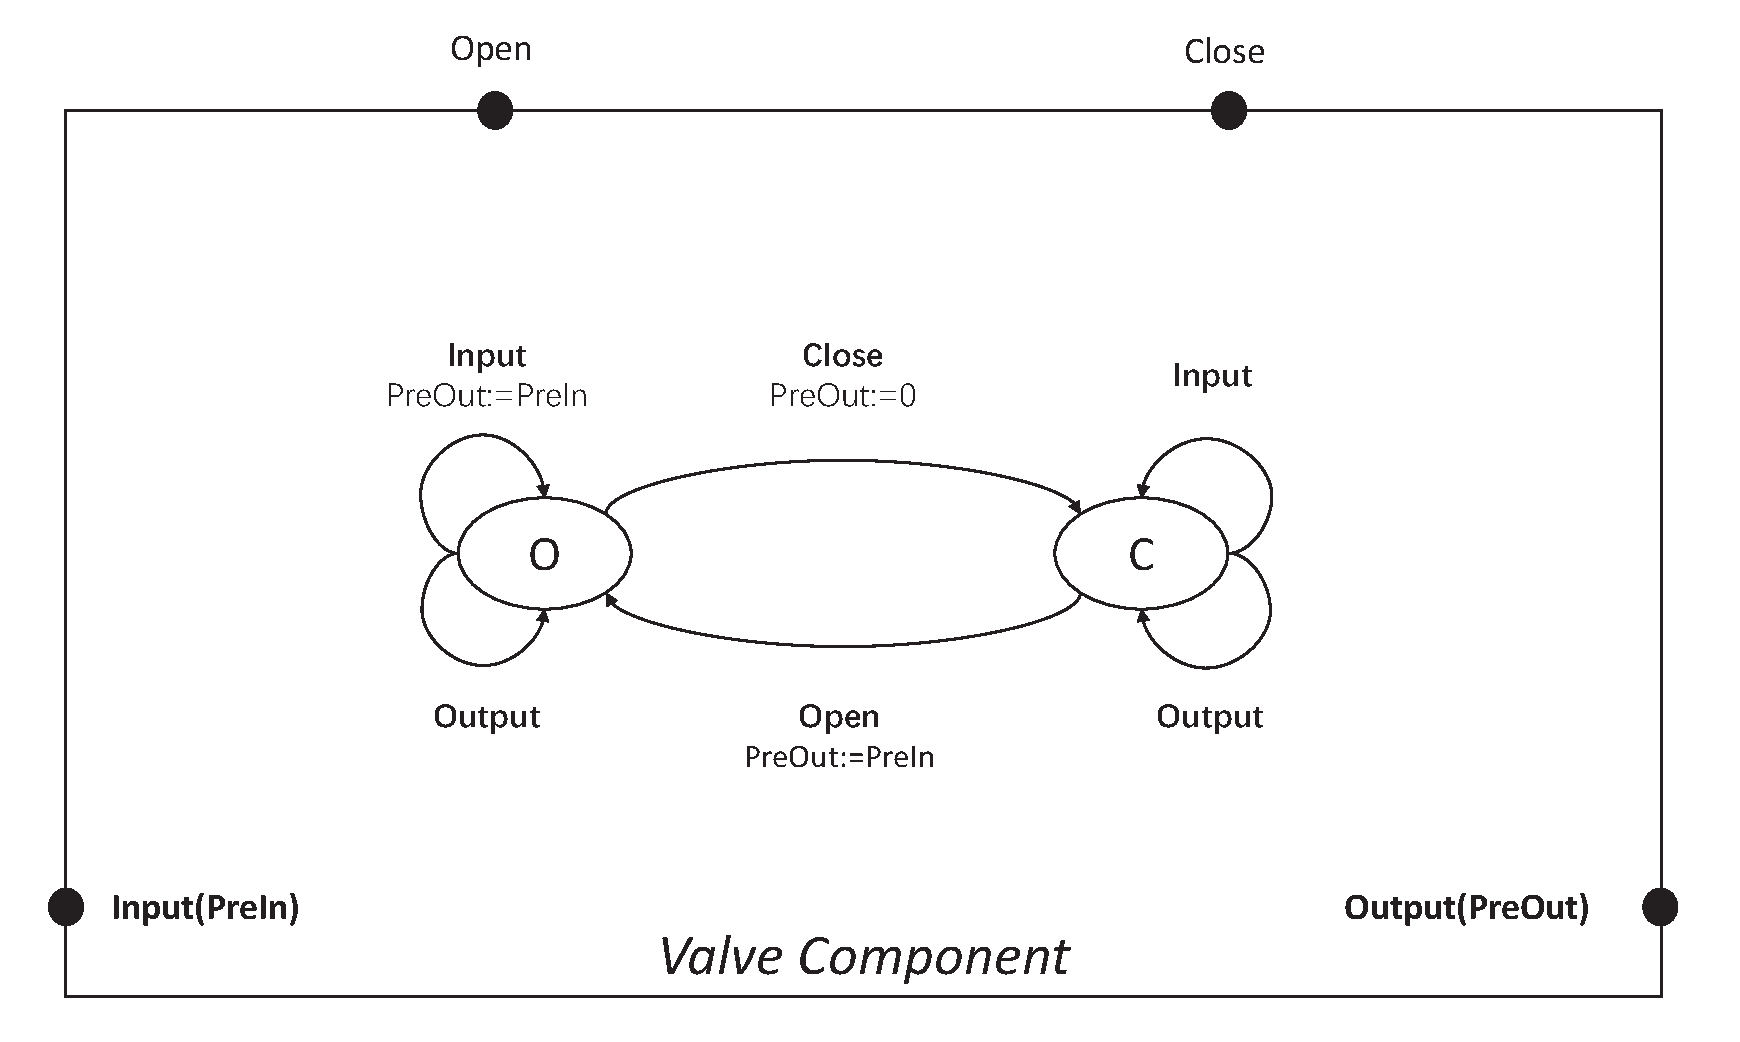
\includegraphics[width=65mm]{figure/example_origin.eps}}
	\caption{The nominal behavior of valve in BIP}
	\label{example_BIP_nominal}
\end{figure}

\begin{comment}
\begin{figure}[htbp]
	\centerline{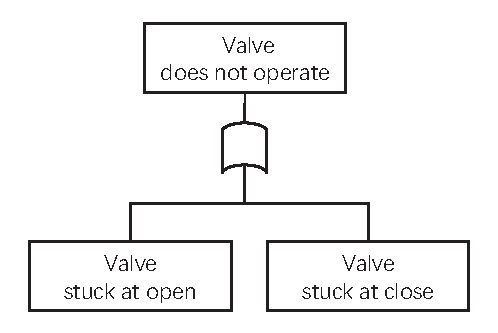
\includegraphics[width=50mm]{figure/example_fault_tree.eps}}
	\caption{Fault tree for a loss of valve occurrence}
	\label{example_valve_fault_tree}
\end{figure}

\begin{figure}[htbp]
	\centering
	\subfigure[pic1.]{
		\begin{minipage}[t]{0.5\linewidth}
			\centering
			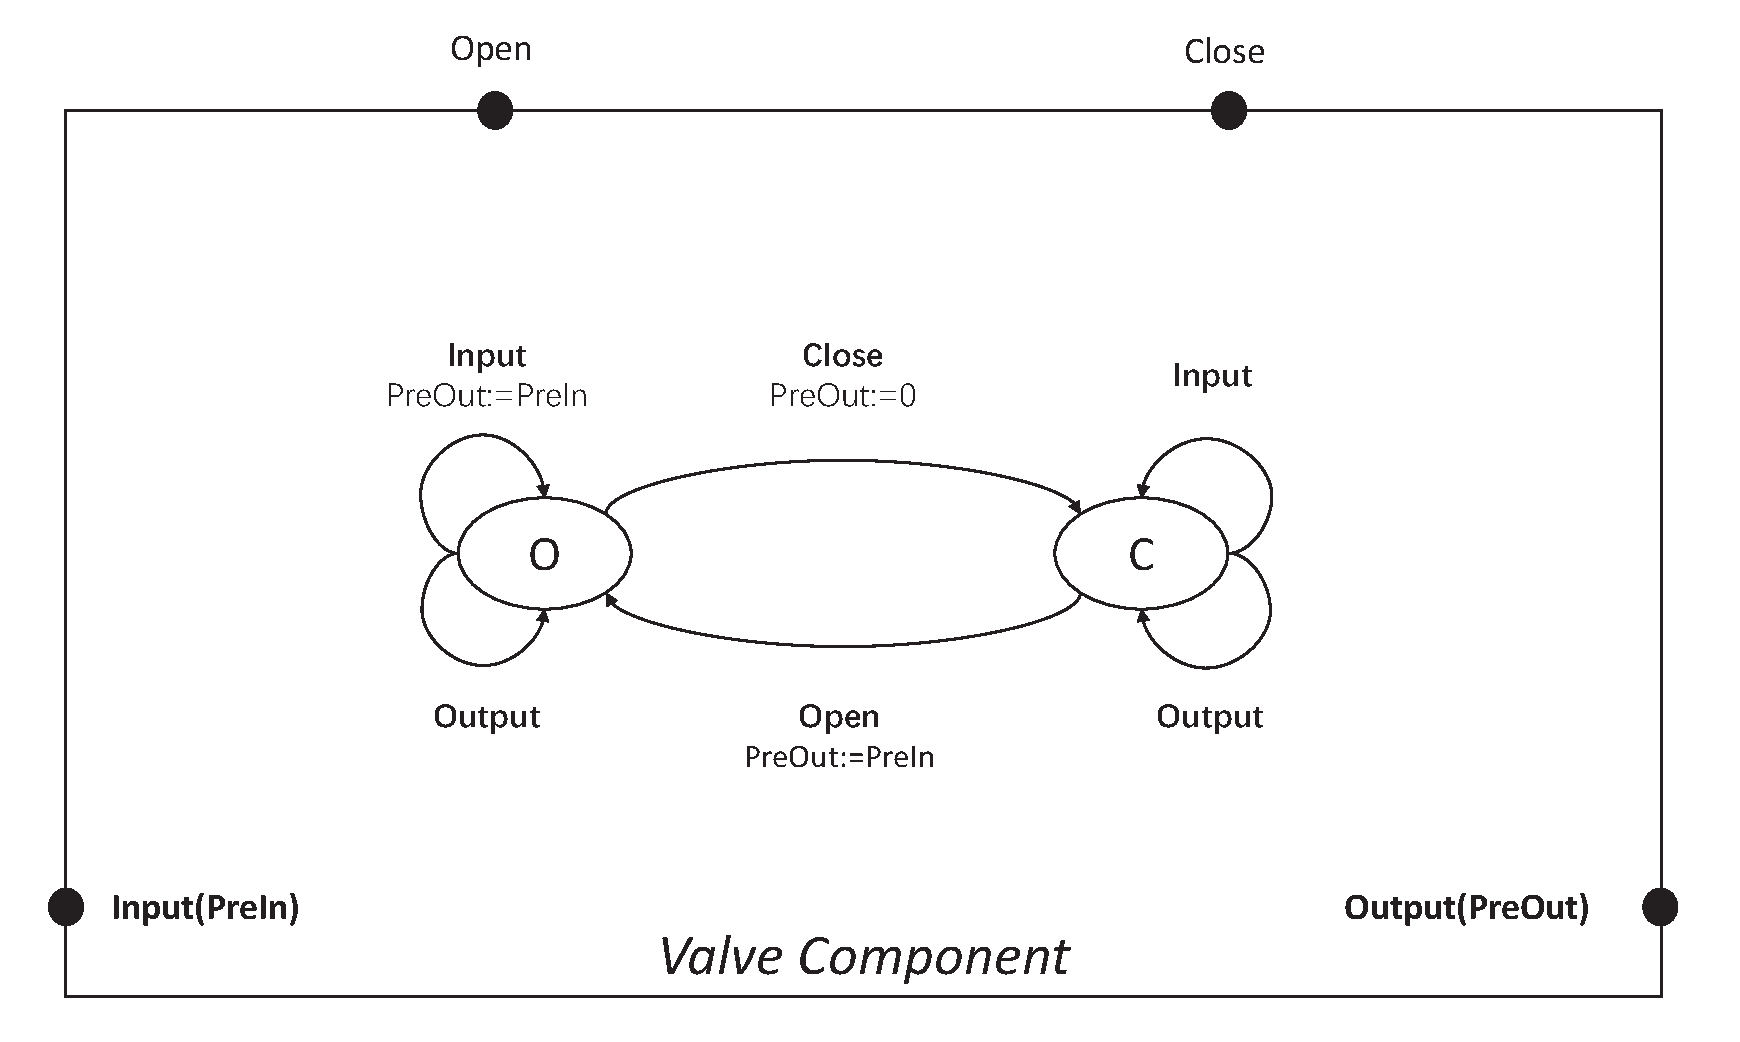
\includegraphics[width=65mm]{figure/example_origin.eps}
			%\caption{fig1}
		\end{minipage}%
	}%
	\subfigure[pic2.]{
		\begin{minipage}[t]{0.5\linewidth}
			\centering
			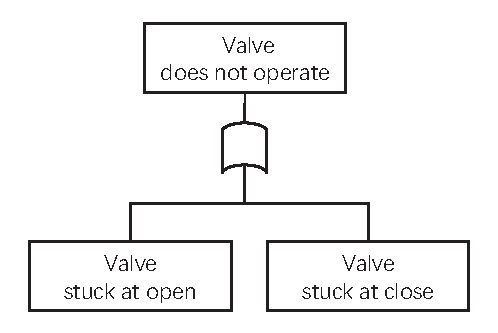
\includegraphics[width=50mm]{figure/example_fault_tree.eps}
			%\caption{fig2}
		\end{minipage}%
	}%
	\centering
	\caption{ pics}
\end{figure}
\end{comment}

%\cite{ft02}

The description of leaf nodes is dependent on the chosen of system tree.
We consider a fault tree that takes the loss of valve as basic fault event.
We subjectively judge that a loss of valve occurs when the valve is stuck at open or it is stuck at close. 
\begin{comment}
We deduce two faulty behaviors for the valve component from the leaf nodes of this fault tree, the stack-at-open fault and stuck-at-close fault. 
\end{comment}
For stuck-at-open fault, the output hydraulic pressure is always the same as the input, while for stuck-at-close fault, the output hydraulic pressure is always zero.

\emph{The integration steps.} We conclude our methodology of integrating the leaf node of fault tree into the valve component shown in Fig.~\ref{example_BIP_nominal} by the following steps:

Step 1: Decompose the fault tree. We pay attention to those basic events which may cause the top level fault. In this example, we consider the loss of valve as leaf node decomposed from the fault tree.

Step 2: Deduce the faulty behaviors from the leaf node. 
We deduce faulty behaviors from the basic event \emph{loss of valve}. We take two faulty behaviors into consideration, they are introduced as follows:

\begin{itemize}
	\item For stuck-at-open fault, the output hydraulic pressure is always the same as the input.
	\item For stuck-at-close fault, the output hydraulic pressure is always zero.
\end{itemize}

Step 3: Generate BIP component with faulty behavior. Comparing with the nominal behavior valve component, the valves with stuck-at-open/close fault show an eternally unblocked/blocked for both \emph{Open} and \emph{Close} status respectively. According to step 3, the faulty behavior valve components are generated as follows:

\begin{itemize}
	\item For both faulty behavior components, the transition among \emph{Open} and \emph{Close} status will no longer change the value of \emph{PreOut}.
	\item For stuck-at-open component, the action of transition from status \emph{Close} to \emph{Close} under event \emph{Input} is \emph{PreOut:=PreIn}, just the same as transition from status \emph{Open} to \emph{Open} under event \emph{Input}.
	\item For stuck-at-close component, the action of transition from status \emph{Open} to \emph{Open} under event \emph{Input} is \emph{PreOut:=0}, just the same as transition from status \emph{Close} to \emph{Close} under event \emph{Input}.
\end{itemize}

Step 4: Design a manager component for deciding and monitoring the activation of both fault and nominal behavior components. In this example, we design a manager component with three states, each of them represents one kind of valve status. Once the state execute a self circulation, an event will be sent to the corresponding behavioral component to activate it. The three states switch through internal port \emph{Trigger} which is controlled by BIP engine to support a stochastic process of faulty behavior occurred during simulation.

Step 5: Since the original component has been integrated with faulty behavior, it keeps the same external port for connection as before but has been extended a lower level to contain various of components designed in the previous steps. Modifying the upward connectors from components to the compound and extending each component with an external port receiving activation event. Confirming the extended system model without fault keeps consistence of the nominal system model through observing their transition of status, internal and external ports and connectors.

%(This will be reconfirmed by tracing the simulation result)

\begin{figure}[t]
	\centerline{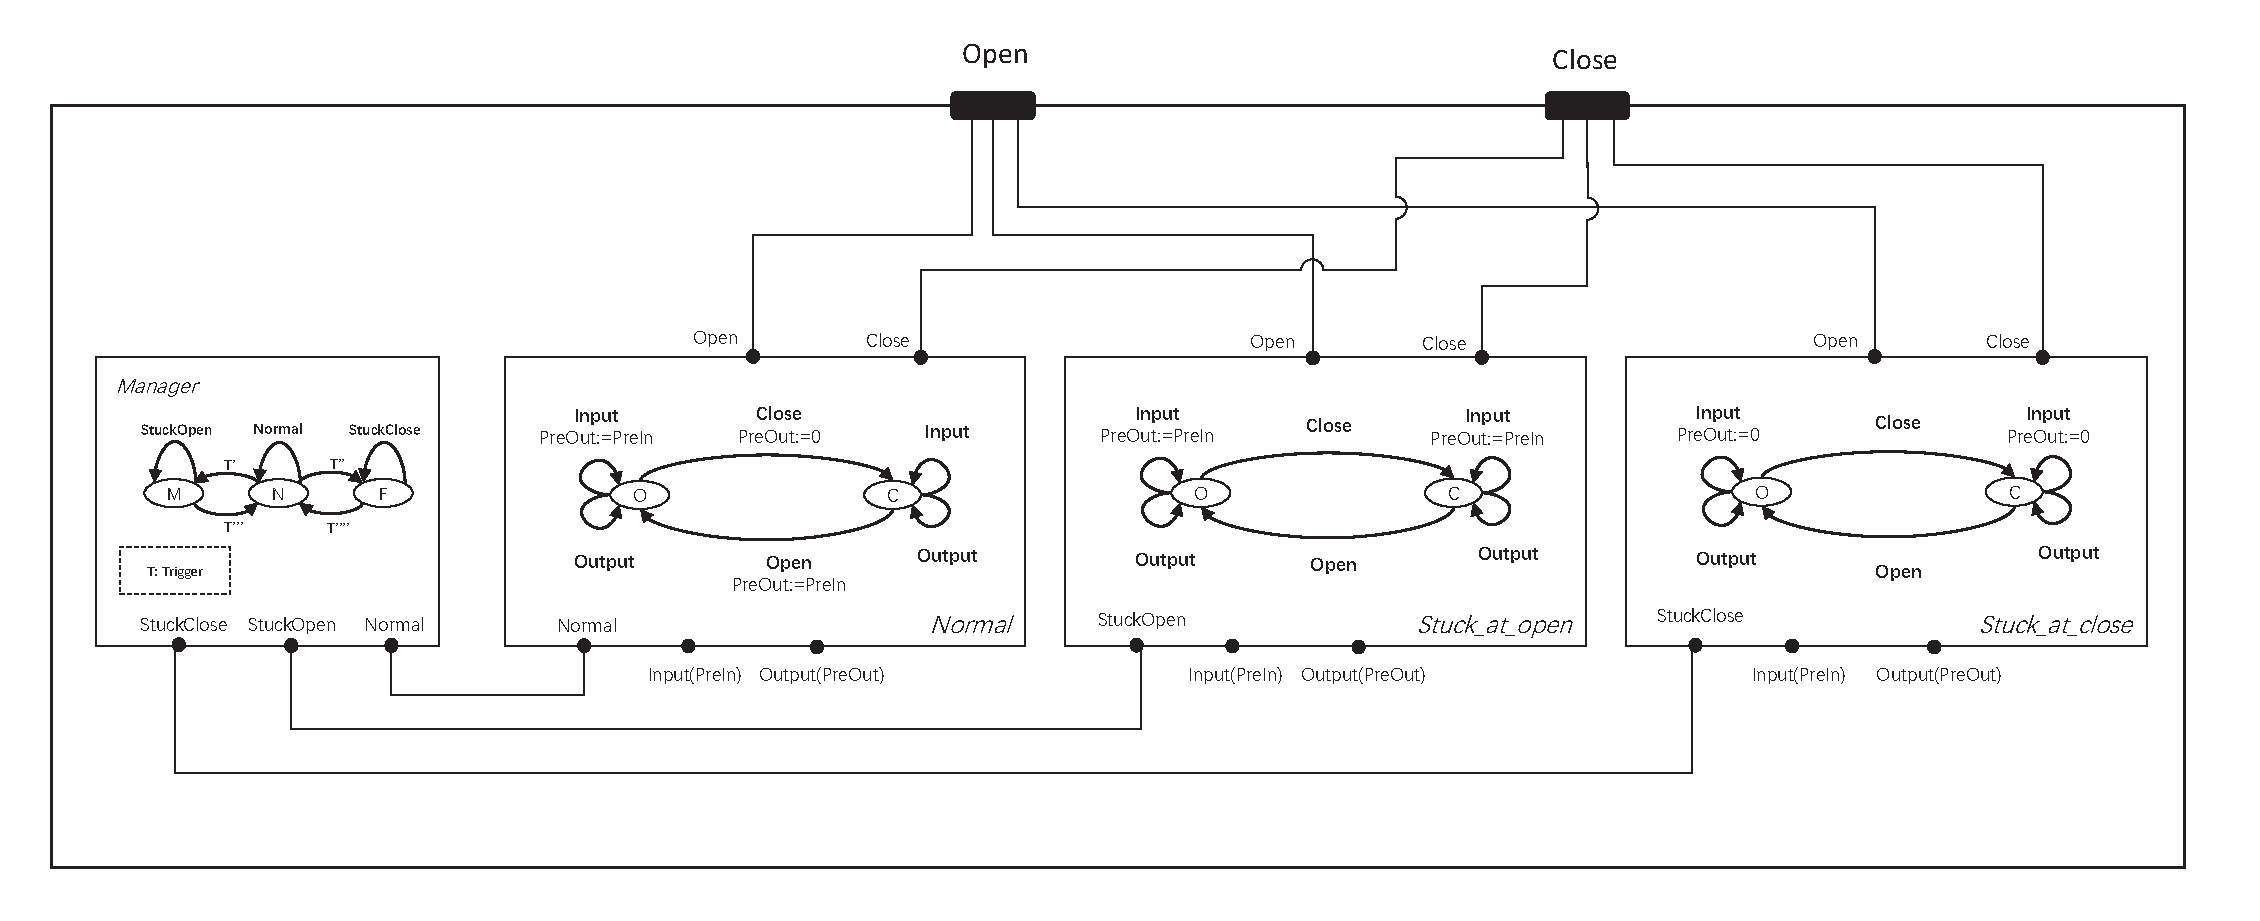
\includegraphics[width=125mm]{figure/Example.eps}}
	\caption{An integration example of common valve component}
	\label{Example}
\end{figure}

As a result of integration, Fig.~\ref{Example} shows the valve compound containing a valve component with nominal behavior, two valve components with faulty behavior and a manager component. Using this BIP model, we integrate failure into the software behavior instead of separating the hardware failure from software system. As hierarchies of complex components, the integrated compound helps us observe the system behavior through graphical representation of BIP model. Also, further simulation and validation of tracing faulty behavior using stochastic BIP engine becomes possible.

% ``Loss of wheel braking" or \emph{Loss of wheel braking}?

\subsection{Fault trees for the WBS}
Fig.~\ref{WBS_BIP_fault_tree} shows a fault tree for ``Loss of wheel braking" event, which is based on the AIR6110 description. Loss of wheel braking is caused either through the Loss of operation of physical system or due to the loss of BSCU. We focus on the leaf nodes which represent faulty behavior for their component respectively. Notice that the expansion of the fault tree nodes ``Loss of BSCU channel 1/2" are carried out but not included in Fig.~\ref{WBS_BIP_fault_tree} for the sake of brevity.

We deduce the faulty behaviors for every component from the fault tree shown in Fig.~\ref{WBS_BIP_fault_tree}. Also, we consider the compound \emph{BSCU Channel 1/2} as the lowest level of component for the sake of brevity. A statistics of deduced faulty behaviors is given in Table.~\ref{tab1}. The selector valve's faulty behavior is loss of its selector function, while each BSCU channel has three faulty behaviors including ``loss of power supply", ``loss of monitor system" and ``command system does not operate".

\begin{figure}[t]
	\centerline{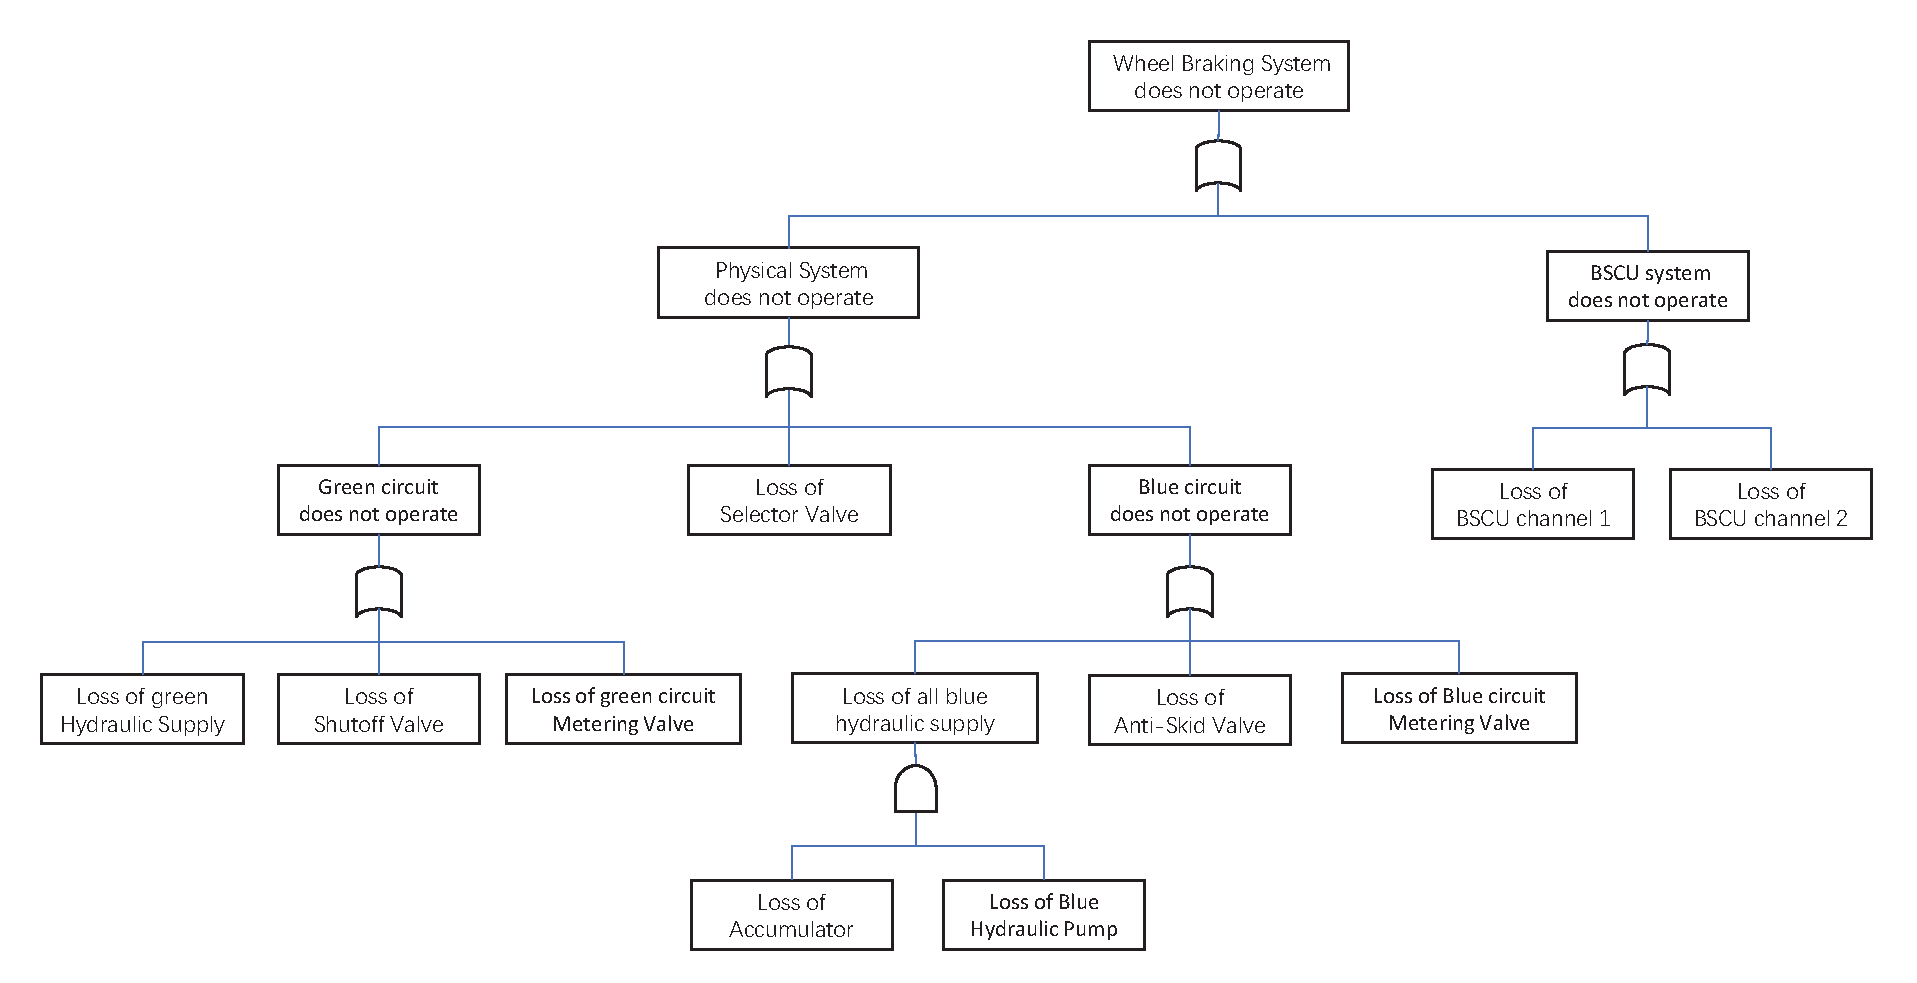
\includegraphics[width=105mm]{figure/fault_tree.eps}}
	\caption{Fault tree for a loss of WBS occurrence under ARCH4}
	\label{WBS_BIP_fault_tree}
\end{figure}

\begin{table}[htbp]
	\caption{Deduced faulty behavior statistics under ARCH4}
	\begin{center}
	\linespread{1.3}\selectfont
		\begin{tabular}{c|c|@{}p{0.002\linewidth}<{\centering}@{}|c}
			\hline
			\multicolumn{2}{c}{Component}&&{Number of fault(s)}\\
			\hline
			\multirow{3}*{\tabincell{c}{Pumps}}&{Green Hydraulic Pump}&&{1}\\
			\cline{2-4}
			&{Blue Hydraulic Pump}&&{1}\\
			\cline{2-4}
			&{Accumulator}&&{1}\\
			\hline
			\multirow{5}*{\tabincell{c}{Valves}}&{Shutoff Valve}&&{2}\\
			\cline{2-4}
			&{Anti-Skid Valve}&&{2}\\
			\cline{2-4}
			&{Green Meter Valve}&&{2}\\
			\cline{2-4}
			&{Blue Meter Valve}&&{2}\\
			\cline{2-4}
			&{Selector Valve}&&{1}\\
			\hline
			\multirow{2}*{BSCU}&{BSCU channel 1}&&{3}\\
			\cline{2-4}
			&{BSCU channel 2}&&{3}\\
			\hline
		\end{tabular}
		\label{tab1}
	\end{center}
\end{table}

\subsection{Extended WBS Model with faults}
In this section, we give a whole view of modified BIP model which is integrated with fault tree introduced in section \emph{5.1} using the methodology provided in section \emph{5.2}.

Table.~\ref{tab2} shows metrics for the different architectures. We focus on observing the diversities between the adjacent architectures and the differences between the nominal system architecture and extended system architecture. The count of max depth of each architecture provides an overview of the usage of hierarchies of complex components. The count of internal ports indicating the number of inner transitions with guard in every component while the count of external ports indicating the number of outer interface of each component.

\begin{table}[t]
	\caption{BIP Nominal/Fault Model statistics}
	\begin{center}
		\linespread{1.3}\selectfont
		\begin{tabular}{c|c|@{}p{0.002\linewidth}<{\centering}@{}|c|c|c|c}
			\cline{4-7}
			\multicolumn{2}{c}{}&&{ARCH1}&{ARCH2}&{ARCH3}&{ARCH4}\\
			\hline
			\multirow{2}*{\tabincell{c}{Component\\types}}&{Nominal}&&{12}&{12}&{15}&{15}\\
			\cline{2-7}
			&{Extended}&&{24}&{24}&{25}&{25}\\
			\hline
			\multirow{2}*{\tabincell{c}{Compound\\types}}&{Nominal}&&{1}&{1}&{2}&{2}\\
			\cline{2-7}
			&{Extended}&&{8}&{8}&{9}&{9}\\
			\hline
			\multirow{2}*{Max depth}&{Nominal}&&{2}&{2}&{3}&{3}\\
			\cline{2-7}
			&{Extended}&&{4}&{4}&{4}&{4}\\
			\hline
			\multirow{2}*{Variables}&{Nominal}&&{38}&{45}&{90}&{91}\\
			\cline{2-7}
			&{Extended}&&{102}&{115}&{134}&{135}\\
			\hline
			\multirow{2}*{\tabincell{c}{Internal\\ports}}&{Nominal}&&{18}&{22}&{30}&{30}\\
			\cline{2-7}
			&{Extended}&&{104}&{114}&{128}&{128}\\
			\hline
			\multirow{2}*{\tabincell{c}{External\\ports}}&{Nominal}&&{33}&{39}&{64}&{65}\\
			\cline{2-7}
			&{Extended}&&{96}&{109}&{126}&{127}\\
			\hline
		\end{tabular}
		\label{tab2}
	\end{center}
\end{table}

We can conclude that the later the design version of the architecture, the greater the scale of the BIP model.
ARCH1 is established as high level architecture without regard to redundancy. Thus, the design of blue hydraulic line and selector valve are not included in ARCH1.
ARCH2, ARCH3 and ARCH4 show large delta comparing with ARCH1.
From ARCH2 to ARCH3, there is a differ from the design for the BSCU.
For ARCH2, the standard only requires a redundency of BSCU which results in a WBS model including two identical BSCU system. For ARCH3, motivated by trade studies on ARCH2, the structure is modified from two BSCUs to a BSCU with dual channels.
Though the decision of dual channels improve the fault tolerance, it increases the number of ports and variables.
ARCH3 and ARCH4 show the closest metrics for the only little change is the input of seletor valve and the location of accumulator.
From another perspective, as the result of integration, the extended BIP model with faulty behavior presents a larger scale than the nominal BIP model.

The graphical representation of the BIP model can separate the correct behavior from the faulty behavior to a great extent. This helps us tracing how a single point of failure impacts the system and whether it will cause a top level failure or not.

%with the faults described in the fault tree in section \emph{B}

The nominal WBS model and the extended model described in this section can be found at \href{https://github.com/Rosaugo/WBSFaultModelingBIP}{https://github.com/Rosaugo/WBSFaultModelingBIP}. 

\begin{comment}
\begin{table}[htbp]
	\caption{BIP Nominal/Fault Model statistics}
	\begin{center}
	\linespread{1.3}\selectfont
\begin{tabular}{c|c|@{}p{0.002\linewidth}<{\centering}@{}|c|c|c|c|}
	\hline
	\multicolumn{2}{c|}{}&&{ARCH1}&{ARCH2}&{ARCH3}&{ARCH4}\\
	\hline
	\multirow{2}*{\tabincell{c}{Component\\types}}&{Nominal}&&{12}&{12}&{15}&{15}\\
	\cline{2-7}
	&{Extended}&&{24}&{24}&{25}&{25}\\
	\hline
	\multirow{2}*{\tabincell{c}{Compound\\types}}&{Nominal}&&{1}&{1}&{2}&{2}\\
	\cline{2-7}
	&{Extended}&&{8}&{8}&{7}&{7}\\
	\hline
	\multirow{2}*{Max depth}&{Nominal}&&{2}&{2}&{3}&{3}\\
	\cline{2-7}
	&{Extended}&&{4}&{4}&{4}&{4}\\
	\hline
	\multirow{2}*{Variables}&{Nominal}&&{38}&{45}&{90}&{91}\\
	\cline{2-7}
	&{Extended}&&{102}&{115}&{134}&{135}\\
	\hline
	\multirow{2}*{\tabincell{c}{Internal\\ports}}&{Nominal}&&{18}&{22}&{30}&{30}\\
	\cline{2-7}
	&{Extended}&&{104}&{114}&{128}&{128}\\
	\hline
	\multirow{2}*{\tabincell{c}{External\\ports}}&{Nominal}&&{33}&{39}&{64}&{65}\\
	\cline{2-7}
	&{Extended}&&{96}&{109}&{126}&{127}\\
	\hline
\end{tabular}
		\label{tab2}
	\end{center}
\end{table}
\end{comment}